\apendice{Documentación de usuario}

\section{Introducción}
En este apendice se detallan los requerimientos de la aplicación, los pasos de instalación, despliegue, así como las indicaciones para su uso adecuado.
\section{Requisitos de usuarios}
Los requesitos para poder hacer uso de la aplicación son:
\begin{itemize}
    \item Tener instalado Python (minimo la version 3.7) y el resto de las librerías contenidas en el \textit{requeriments.txt}.
    \item Tener un navegador web compatible con HTML5 
\end{itemize}

\section{Instalación}
Para la instalación en local de la aplicación, deberemos descargarnos el contenido del repositorio (\url{https://github.com/mtc1003/TF_Keras_TFG}).
Para ello podremos seguir una de las opciones vistas en \ref{downloadGit}, tras esto, deberemos de desplazarnos al interior de la carpeta \textit{codigo/yolov4ToTensorFlow} y desde ahi, instalar las dependencias de la aplicación, ya sea mediante el fichero de dependencias de Anaconda o mediante el fichero de \textit{requeriments}.
Tras esto podremos levantar la aplciacion ejecutando el fichero \textit{app.py} o mediante el comando Flask run, levantadose de ambas maneras la aplicación.

\section{Manual del usuario}
En esta sección se explicarán las diferentes tareas que puede hacer un usario en la aplicación.
\imagen{homeAPP}{\textit{Home} de la aplicación}
\subsection{Carga de modelo de detección}
Esta opción se encuentra en el \textit{home} de la aplicación, correspondiendose esta opción con el primer botón, al hacer \textit{click} sobre él se nos abrirá una modal, la cuál cuenta con dos inputs, uno de tipo text y otro de tipo file(este posee funcionalidad de \textit{click} y de \textit{drag and drop}).
\begin{figure}[!h]
    \centering
    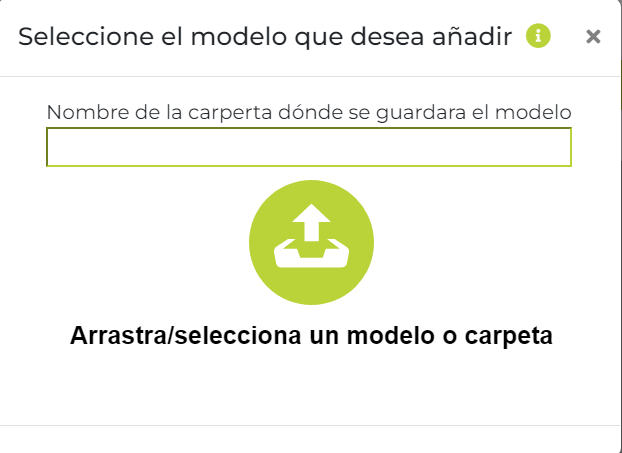
\includegraphics[width=0.6\textwidth]{modalModel}
    \caption{Modal para añadir modelos}\label{fig:modalModel}
\end{figure}
El input de tipo \textit{text}, sirve para introducir el nombre de la carpeta en la cuál se guardará el modelo de detección, de tal forma que sea más fácil encontrarlo posteriormente.
En segundo input de tipo \textit{file}, nos permite escoger el modelo que queremos añadir a la aplicación, ya sea un modelo de \textit{Tensorflow Lite} o una carpeta con el modelo de \textit{Tensorflow}. Ver Imagen \ref{fig:modalModel}

\subsection{Carga de fichero de etiquetas}
Está opción se corresponde con el segundo botón de acciones del \textit{home}, al hacer \textit{click} sobre él se abrirá una modal, la cuál, es de un estilo similar a la modal de añadir modelos, en está encontraremos un input de tipo \textit{file}, el cuál funciona sólo por \textit{click}, el cuál permite la carga de archivos cuya extensión sea \textit{names}. Ver Imagen \ref{fig:modalNames}
\begin{figure}[!h]
    \centering
    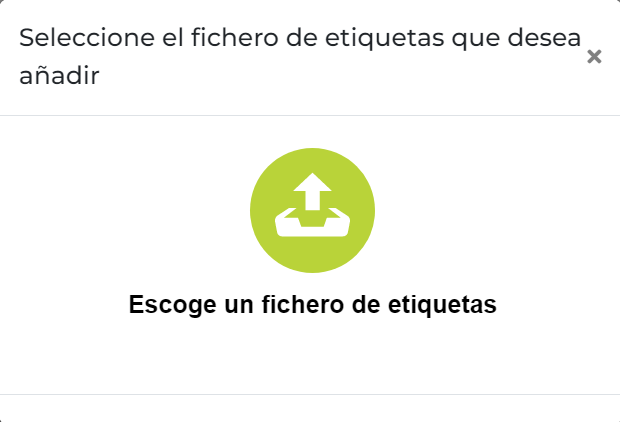
\includegraphics[width=0.6\textwidth]{modalNames}
    \caption{Modal para añadir ficheros de etiquetas}\label{fig:modalNames}
\end{figure}

\subsection{Cambiar fichero de etiquetas} \label{Cambiar fichero de etiquetas}
Esta opción, al igual que las dos anteriores, se encuentra en el \textit{home}, concretamente es el tercero de los botones de acciones, al hacer \textit{click} sobre él, se abrirá una ventana modal, la cuál posee el listado de todos los ficheros de etiquetas que posee la aplicación, encontrándose en cada acceso el fichero de etiquetas que se encuentra seleccionado (ver Imagen \ref{fig:selectNames}).
Para realizar un cambio de fichero, se debe de hacer \textit{click} en listado de los fichero, el cuál desplegara todos los los fichero que se encuentran en la aplicación, se selecciona el fichero con el que deseamos trabajar y hacemos \textit{click} en botón de \textbf{Cambiar fichero}.

\begin{figure}[!h]
    \centering
    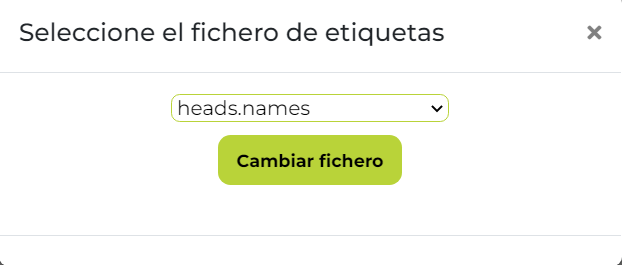
\includegraphics[width=0.6\textwidth]{selectNames}
    \caption{Modal para cambiar ficheros de etiquetas}\label{fig:selectNames}
\end{figure}

En el momento en el que se realice el cambio se mostrará el siguiente mensaje de confirmación (Ver Imagen: \ref{fig:OKSelectNames}) y tras su cierre se veremos como opción seleccionada el nuevo fichero de etiquetas.

\begin{figure}[!h]
    \centering
    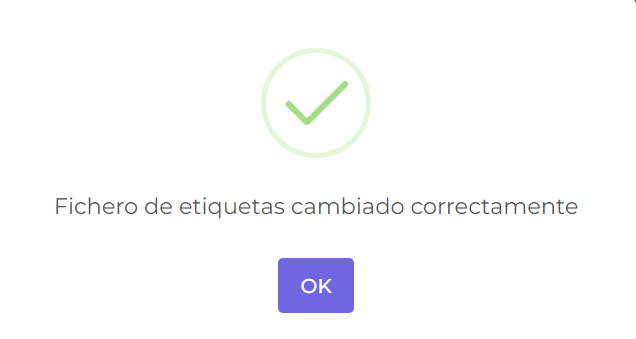
\includegraphics[width=0.6\textwidth]{OKSelectNames}
    \caption{Mensaje de confirmación de que el fichero de etiquetas se ha cambiado correctamente}\label{fig:OKSelectNames}
\end{figure}

\subsection{Cambiar modelo de detección}
Para llevar a cabo esta opción de la aplicación, se debe de hacer \textit{click} en el cuarto botón del listado de botones de acciones, el cuál abrirá una ventana modal, que contiene un menú de selección con todos los modelos que se encuentran en la aplicación(tanto modelos de Tensorflow(formato \textit{pb}) como modelos de Tensorflow Lite).

\begin{figure}[!h]
    \centering
    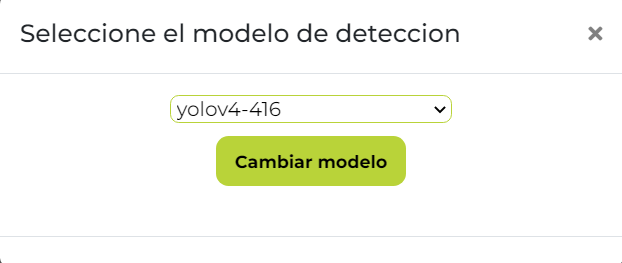
\includegraphics[width=0.6\textwidth]{selectModel}
    \caption{Modal para cambiar modelos de etiquetas}\label{fig:selectModel}
\end{figure}

La funcionalidad de esta modal es muy similar a la modal \ref{Cambiar fichero de etiquetas}, en la cuál se encuentra seleccionado, al hacer \textit{click} sobre el listado de selección se mostrará todos los modelos que hay en la aplicación, para cambiar de modelo, tan sólo tendremos que cambiar el modelo seleccionado haciendo \textit{click} en la lista y escoger el modelo con el que deseamos trabajar.
El proceso del cambio tarda uno segundos, ya que, nos deja el modelo plenamente funcional para trabjar con él.

\subsection{Detección de objetos en una imagen} \label{od_img}
Esta opción se corresponde con la primera imagen de las seis que hay en el menú de detecciones.

\imagen{homeDetect}{Menú de detecciones}

Esta opción nos permite detectar objetos sobre una imagen, para ello debemos partir de un modelo y de un fichero de etiquetas seleccionado.
Al hacer \textit{click} sobre la imagen nos llevará a una nueva ventana, en la cuál podremos ver (al igual que en el homme), el modelo y el fichero de etiquetas seleccionado, 
a su vez, en la esquina superior izquierda un botón, <- volver al home, el cuál nos permite regresar al menú \textit{home}.

\imagen{odImg}{Página de detección de Objetos sobre una imagen}

Al hacer \textit{click} sobre el input, seleccionaremos la imagen la cuál deseamos etiquetar sus elementos, la cuál se nos mostrará en previsualización y nos "desbloqueará" un botón que nos permite detectar los objetos en la imagen.

\imagen{preDetectImg}{Imagen cargada para ser detectada}

Al hacer \textit{click} en \textbf{Detectar}, comenzará el proceso de detección y al acabar nos mostrará la imagen etiquetada, así como dos links de descarga(uno para la imagen etiquetada y otro para el fichero CSV de posiciones).

\imagen{posODImg}{Resultado de la detección en una imagen}

\subsection{Detección de objetos en un vídeo} \label{odVideo}
Esta opción se corresponde con la segunda de la opciones del menú de detecciones, la cuál nos permite detectar objetos sobre un vídeo.
Esta página posee los msimos datos informativos que la opción de \textbf{Detección de objetos en una imagen}(modelo de detección actual, modelo de detección actual y el botón de vuelta al home).

\imagen{odVideo}{Página de detección de Objetos sobre un vídeo}

La funcionalidad de esta opción es igual que la de detección en imagen (Ver \ref{od_img}), pero en lugar de seleccionar una imagen, se selecciona un vídeo.
El cuál, en cuanto se carga se previsualiza, permitiendonos reproducirlo. Al inicio de la detección, se nos mostrará el mensaje "Detectando... Si desea detener la detección pulse la tecla Q", de tal forma, que si deseamos parar la detección porque el vídeo es demasiado largo, 
o porque no nos interesá detectar todo el vídeo, podamos hacerlo y ver el resultado de la detección hasta ese punto. Al acabar la detección, podremos descargar el vídeo etiquetado y el fichero CSV de posiciones.

\begin{figure}[!h]
    \centering
    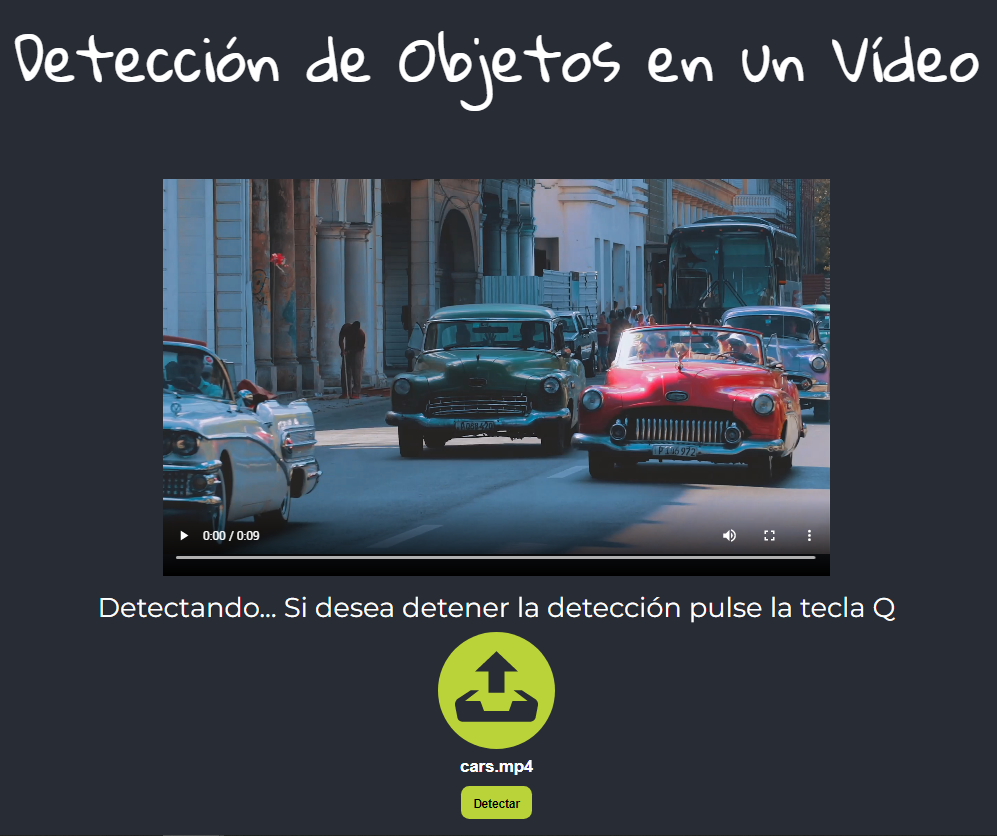
\includegraphics[width=0.6\textwidth]{stopOD}
    \caption{Proceso de detección de objetos en un vídeo}\label{fig:stopOD}
\end{figure}

\begin{figure}[!h]
    \centering
    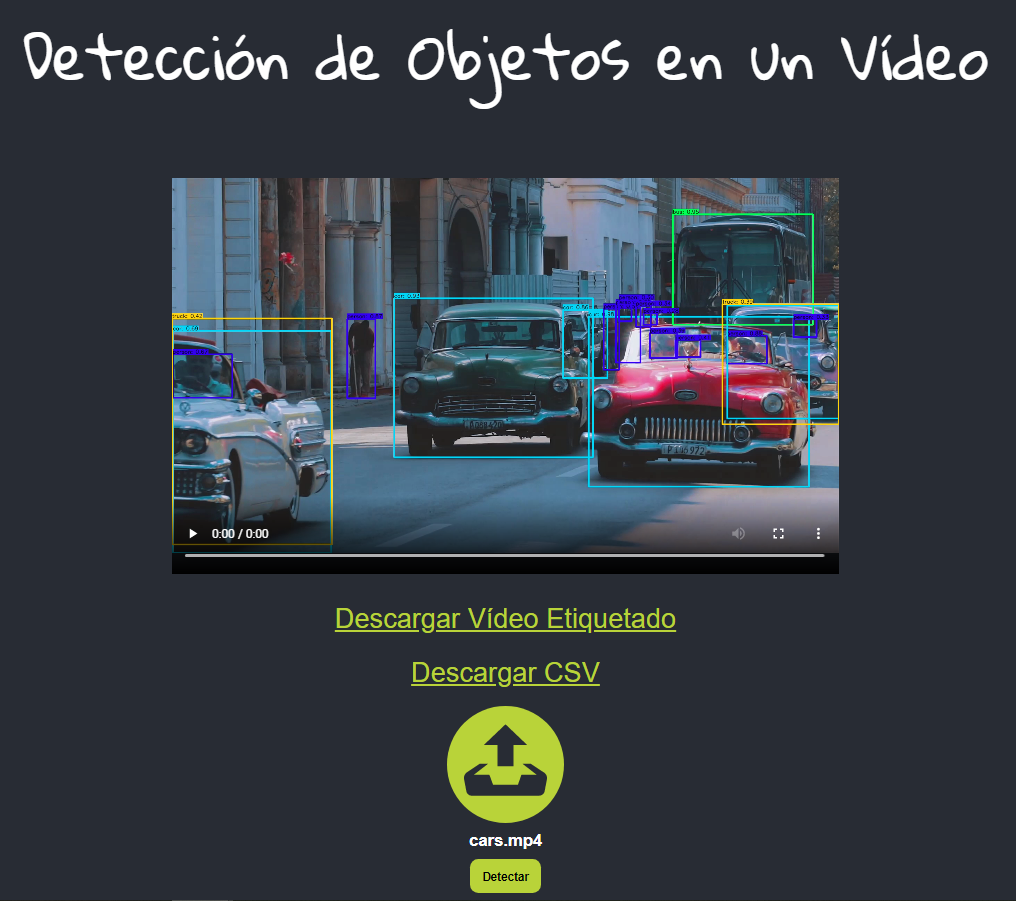
\includegraphics[width=0.6\textwidth]{odVideoEnd}
    \caption{Detección sobre vídeo teminada/detenida}\label{fig:odVideoEnd}
\end{figure}

\subsection{Contabilizar objetos en un vídeo} \label{odTrack}
Esta opción, se corresponde con la tercera opción del menú de detecciones, está funciona de la misma manera que \ref{odVideo}, deberemos seleccionar un vídeo en cuál se contabilizan los diferentes objetos que se encuentran en el vídeo.
Es decir, son dos opciones que s simple vista, funcioan exactamente igusl, pero realizan funciones de detección diferentes.

\subsection{Detección de objetos a tráves de la URL de una imagen} \label{odURl}
Esta opción es la cuarta de la lista de opciones de detección, la cuál nos permite detectar objetos sobre la url de una imagen, es decir, la detección se lleva a cabo sobre una imagen de Internet.

\imagen{odURL}{Detección de objetos sobre la URL de una imagen}

Para llevar a cabo la detección, deberemos de copiar la \textit{URL} de la imagen en el cuadro de texto, en el momento en el que el input detecte el contenid, nos mostrará el boton de \textbf{Detectar}.
Al hacer \textit{click} en el botón de \textbf{Detectar} comenzará el proceso de detección, lo cuál nos delvolverá un resultado correcto, siempre y cuándo la URL de la imagen poseea un \textit{.es} o un \textit{.com}.
Al acabar la detección, podremos descargar la imagen etiquetada y el fichero CSV de posiciones.

\imagen{odURLEnd}{Resultado de la detección a tráves de la URL de la imagen}

\subsection{Detección de objetos a tráves de la URL de un vídeo de YouTube}
Esta opción es la quinta del menú de detecciones, al igual que la función \ref{odURl} trabajan sobre las URLs de los objetos, pero esta trabaja sobre la \textit{url} de un vídeo de YouTube (es importante que esta url se obtenga desde la opción de compartir vídeo, y desde ahí copiar link, ya que de otra manera la detección nos daría error).
Al acabar la detección, podremos descargar el vídeo etiquetado y la fichero CSV de posiciones.

\imagen{odURL-YT}{Detección de objetos sobre la URL de un vídeo YouTube}

Al introducir la \textit{url}, dos mostrará el botón \textbf{Detectar} y al hacer \textit{click} sobre él, comezará el proceso de detección, al inicio de la detección
se nos mostrará el mensaje "Leyendo el vídeo de YouTube" ver imagen \ref{lvYT} y seguidamente "Detectando... Si desea detener la detección pulse la tecla Q", pudiendo detener la detección en cualquier momento, de la misma forma que en las opciones \ref{odVideo} y \ref{odTrack}.

\imagen{lvURL}{Leyendo el vídeo desde YouTube}
\imagen{resultOD-YT}{Resultado de la detección del vídeo de YouTube}

\subsection{Detección de objetos a tráves de webcam}
Esta opción es la última de las posibles opciones de detección, la cuál se encarga de detectar objetos a tráves de la \textit{webcam}, para esta opción es necesario poseer una cámara web.

\imagen{odWbcm}{Página de detección de objetos desde la Webcam}

Esta opción permite detectar objetos desde la \textit{webcam} sin que se grabe el vídeo, es decir, vemos el resultado en vivo pero no obtendremos, la opción de poder descargar el vídeo etiquetado, por otro lado, tendremos la opción de grabar el vídeo etiquetado para su posterior descarga.